\section{Hashing}

\subsection{Definitions}

A hash is a function $h$ that takes the key $k$ to its hash table position $h(k)$.  The universe of keys is large, and the table is much smaller, so $h:U \to T$ is not invertable.   Collisions, where $h(k_i) = h(k_j)$, are possible, so a hash method must have a method of resolving collisions.  

With chaining, each slot in the hash table is actually a linked list of the elements of $U$ hashed to that table position.  The assumption of {\it simple uniform hashing} is that any given element is equally likely to hash into any of the $m$ table slots, independent of where any other element has hashed to.  Let $m = |T|$ and $n$ is the number of elements to be put in the table.  The expected value of the number of elements in linked list $T_i$ is $n/m$.  In a hash table in which collisions are solved by chaining, an unsuccessful search takes average-case time $\Theta(1 + n/m)$ under the assumption of simple uniform hashing.  

\subsection{Examples of Hash Functions}

\begin{description}
	\item [Division] $h(k) = k \pmod m$.  Choose $m$ prime not close to a power of 2.
	\item [Multiplication] $h(k) = \lfloor  m\cdot (\text{fractional part of }kA) \rfloor$ where $A \in (0,1)$ and $m = |T|$.  
	
	Method
	\begin{itemize}
		\item $m = 2^p$
		\item $w = \text{word size (bits)}$, assume $k < 2^w$.
		\item $A = s/2^w$, $0 < s < 2^w$
		\item Multiply $k$ by $s = A \cdot 2^w$.
		\item $ks = r_1 2^w + r_0$
		\item Extract the $p$ most significant digits of $ks$ to be $h(k)$.  
	\end{itemize}
	
	We restrict $A$ to be a fraction of the form $s/2^w$, where $w$ is the word size.  
\end{description}

\subsection{Collision Resolution}

\begin{description}
	\item [Chaining]  Each slot in the hash table is actually a linked list.  
\end{description}

\subsection{Cuckoo Hashing:  NOT IN TEXTBOOK}

Cuckoo hashing is a scheme in computer programming for resolving hash collisions of values of hash functions in a table, with worst-case constant lookup time. The name derives from the behavior of some species of cuckoo, where the cuckoo chick pushes the other eggs or young out of the nest when it hatches; analogously, inserting a new key into a cuckoo hashing table may push an older key to a different location in the table. [Wikipedia]

\

Have two hash tables, each with a different hashing function.  When hashing a key $k$, if $h_1(k)$ is empty in the first table, put it there.  If another key, $k_1$, is there, push it into the second table in $h_2(k_1)$.  and put $k$ in $h_1(k)$.  If $h_2(k_1)$ is full with $k_3$, push $k_3$ into the first table in $h_1(k_3)$.  Continue until there's an empty cell.  

\subsection{Perfect Hashing}

Perfect hashing is for situations where the keys are static, as in the reserved terms in a programming language or the TOC of a DVD.  

Instead of making a linked list for keys hashing to slot $j$, make a secondary hash table $S_j$ with an associated hash function $h_j$.  The size $m_j$ of the secondary hash table has to be the square of the number $n_j$ of keys hashing to slot $j$.  

%%%%%%%%%%
\subsection{Old Exam Questions}

%%%%%
\subsubsection{Spring 2019 \#S2}

	% S19 S2
The hash table is a widely adopted data structure.  Explain briefly how perfect hashing works.  Separately, what is the situation when a new key cannot be inserted in a Cuckoo hash table separately?

\subsubsection{Solution}

Perfect hashing:  Let $m$ be the size of the hash table $T$, and $m_j$ be the number of keys hashed to element $j$ of the hash table.  For each element $j$ of the table, instead of having a linked list to store the $m_j$ elements, have another hash table of size $m_j^2$ to hash them with hash function $h_j$.  It is possible to create each of the hash functions $h_j$ so that there are no collisions within that table.  

A cuckoo hash table is actually two hash tables, $T_1$ and $T_2$ with hash functions $h_1$ and $h_2$.  When hashing a key $k$, if $h_1(k)$ is full, put $k$ there, and hash the pushed-out key into the other table.  If that slot is full, continue pushing keys between the tables until there is an empty slot.  


%%%%%
\subsubsection{Fall 2018 \#S5}

	% F18 #S5
The utilization efficiency of a hash table depends heavily on its hashing function(s) employed.  Describe with a diagram to illustrate how a multiplication method of hashing functions works on a machine with the word size of $w$ bits for a hash table with $2^p$ entries, $p<w$.  

\subsubsection{Solution}

This problem refers to Figure 11.4 on page 264.  

\begin{enumerate}
	\item Let $k$ be the key to be hashed, and $h(k)$ be the hash table value in which we will place $k$.  Assume $k < 2^w$.    
	\item Choose $A \in (0,1)$, by which we really mean choose $s = A \cdot 2^w$.
	\item Multiply $sk$ to get a value of $2w$ bits, $r_1 \cdot 2^w + r_0$.  
	\item Take the $p$ higher-order bits of $r_0$ to be $h(k)$.  
\end{enumerate}

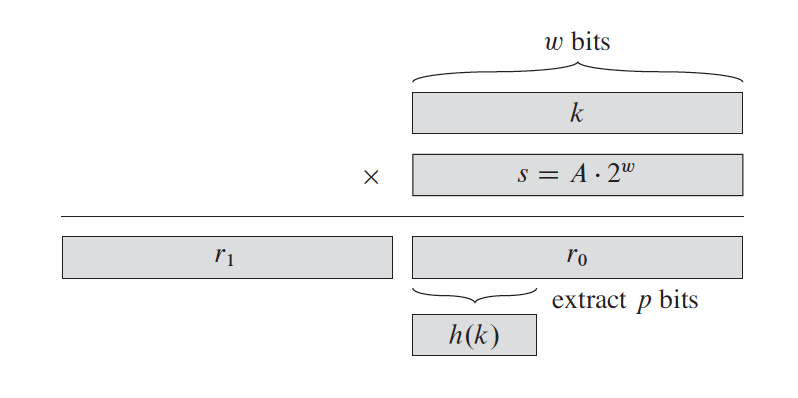
\includegraphics[width=4in]{Cormen_Figure_11_4.png}

%%%%%
\subsubsection{Spring 2018 \#S2}

	% S18 #S2
Given that for an open-address hash table with load factor $\displaystyle \alpha = \frac{n}{m} < 1$, the expected number of probes in unsuccessful search under uniform hashing is at most $\displaystyle \frac{1}{1-\alpha}$, how do you prove the expected number of probes in a successful probe under uniform hashing being at most $\displaystyle \frac{1}{\alpha} \ln \left( \frac{1}{1-\alpha}\right)$?  (Just give a proof sketch, explaining how many probes are needed to locate existing keys.)

\subsubsection{Solution}

This one requires summing probabilities.  I'm going to pass on this one.  

%%%%%
\subsubsection{Fall 2016 \#S9}

	% F16 #S9
Given two hash functions $h_1$ and $h_2$ for Cuckoo hashing under two tables, $T_1$ and $T_2$, 
	\begin{itemize}
		\item Describe the steps involved in inserting a record with the key of $k_{new}$.
		\item Cuckoo hashing can be analyzed by the Cuckoo graph, whose nodes denote table entries and links connect pairs of nodes where given keys can be held.  State when a new key can be inserted successfully based on the Cuckoo graph.
	\end{itemize}

\subsubsection{Solution}

\begin{itemize}
	\item (See above, Spring 2019 \#S2.b)
	\item A new item can be successfully inserted when the Cuckoo graph is acyclic.  
\end{itemize}


%%%%%
\subsubsection{Fall 2015 \#L1}

	% F15 # L1
The utilization efficiency of a hash table depends on its hashing function(s) employed.  Describe with a diagram to illustrate how a multiplication method of hashing works on a machine with word size of $w$ bits for a hash table with $2^p$ entries, $p<w$.  Explain briefly how Cuckoo hashing works under two hash functions of $h_1$ and $h_2$.

\

[Solutions above.]



